\chapter{Vorlesung 07 - 04.12.2025}
\section{Exact reconstruction of additive trees}
Idea: iteratively adding taxa
\subsection*{Example}
\begin{figure}[H]
    \centering
    \begin{subfigure}{0.4\textwidth}
    \centering
     \begin{tikzpicture}
       \draw[fill=black] (-2,0) circle[radius=0.1];
       \node [label=above:$i$] (i) at (-2,0) {};
       \draw[fill=black] (2,0) circle[radius=0.1];
       \node [label=above:$j$] (j) at (2,0) {};
       %\draw[fill=black] (0,-1) circle[radius=0.1];
      % \node [label=above:$v$] (v) at (0,-1) {};
       \draw[fill=black] (0,-3) circle[radius=0.1];
       \node [label=below:$k$] (k) at (0,-3) {}; 
       \path (i) edge (j);
     \end{tikzpicture}
     \caption{Caption}
    \end{subfigure}
    \caption{Caption}
    \label{fig:my_label}
\end{figure}

\begin{figure}[H]
    \centering
   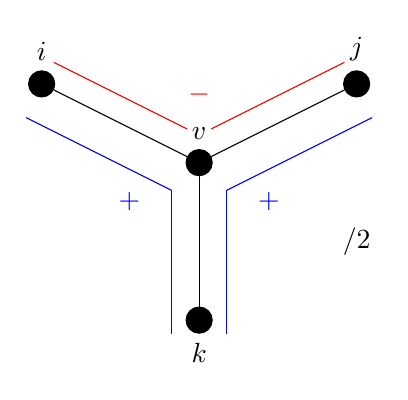
\begin{tikzpicture}
    \node [circle, draw, minimum size=1mm, label=above:$i$,  fill=black] (i) at (-2,0) {};
    \node [circle, draw, minimum size=1mm, label=above:$j$,  fill=black] (j) at (2,0) {};
    \node [circle, draw, minimum size=1mm, label=above:$v$,  fill=black] (v) at (0,-1) {};
    \node [label=above:{\textcolor{red}{$-$}}] (vm) at (0,-0.5) {};
    \node [label=left:{\textcolor{blue}{$+$}}] (vp1) at (-0.5,-1.5) {};
    \node [label=right:{\textcolor{blue}{$+$}}] (vp2) at (0.5,-1.5) {};
    \node [circle, draw, minimum size=1mm, label=below:$k$,  fill=black] (k) at (0,-3) {};
    \node (vp2) at (2,-2) {$/ 2$};
    
    \path[black]  
                (i) edge (v)
                (j) edge (v)
                (k) edge (v);
    \path[red, transform canvas={yshift=10pt}]
                (i) edge (v)
                (j) edge (v);
    \path[blue, transform canvas={yshift=-10pt, xshift=10pt}]
                (j) edge (0,-1)
                (k) edge (0,-1);
     \path[blue, transform canvas={yshift=-10pt, xshift=-10pt}]
                (i) edge (0,-1)
                (k) edge (0,-1);
\end{tikzpicture}
    \caption{Tipp für Klausur: sich einfach das hier merken.}
    \label{fig:my_label}
\end{figure}